\section{Algebraic Structures}

\bd [Algebraic Structures]
A set $A$ (called the underlying set, carrier set or domain), together with a collection of maps (called operations) on $A$ of finite arity (typically binary operations), and a finite set of identities, known as axioms, that these operations must satisfy, is called an \textbf{algebraic structure}. Some algebraic structures also involve another set (called the scalar set).
\ed

Examples of algebraic structures with a single underlying set include groups,fields and rings. Examples of algebraic structures with two underlying sets include vector spaces, modules, and algebras. In this section we will review the most important algebraic structures for our purposes. \\

One has to be careful with the terminology since it changes depending on the area of mathematics. For example, in the context of universal algebra, the set $A$ with this structure is called an algebra, while, in other contexts, it is (somewhat ambiguously) called an algebraic structure, the term algebra being reserved for specific algebraic structures that are vector spaces over a field or modules over a commutative ring. \\

The properties of specific algebraic structures are studied in abstract algebra. The general theory of algebraic structures has been formalized in universal algebra. The language of category theory is used to express and study relationships between different classes of algebraic and non-algebraic objects. This is because it is sometimes possible to find strong connections between some classes of objects, sometimes of different kinds. For example, Galois theory establishes a connection between certain fields and groups: two algebraic structures of different kinds.

\section{Groups}

\bd [Group]
A \textbf{group}\index{field (algebraic)} is a tuple $(G,\cdot)$, where $G$ is a set (called the underlying set of the group) and $\cdot$ is a map (called operation) $G\times G \to G$ satisfying the following four group axioms:
\begin{itemize}
\item Closure: $\forall \, a,b \in G : a \cdot b \in G$;
\item Associativity: $\forall \, a,b,c \in G : (a \cdot b) \cdot c=a \cdot (b \cdot c)$;
\item Neutral Element: $\exists \, e \in G : \forall \, a \in G : a \cdot e = e \cdot a=a$;
\item Inverse Element: $\forall \, a \in G : \exists \, a^{-1} \in G : a \cdot a^{-1} =a^{-1}  \cdot a = e$;
\end{itemize}
\ed

The identity element $e$ of a group $G$ is often written as $1$ a notation inherited from the multiplicative identity. If a group is abelian, then one may choose to denote the group operation by $+$ and the identity element by $0$.\\

The result of the group operation may depend on the order of the operands. In other words, the result of combining element $a$ with element $b$ need not yield the same result as combining element $b$ with element $a$, so the equation $a \cdot b = b \cdot a$ may not be true for every two elements $a$ and $b$.

\bd [Abelian Group]
A group $G$ is called \textbf{Abelian} if on top of the four group axioms it also satisfies the axiom of commutativity:
\begin{itemize}
\item Commutativity: $\forall \, a,b \in G : a \cdot b = b \cdot a$;
\end{itemize}
\ed

Commutativity always holds in the group of integers under addition, because $a + b = b + a$ for any two integers (commutativity of addition). The symmetry group is an example of a group that is not abelian.

\section{Fields}

\bd [Field]
An \textbf{(algebraic) field}\index{field (algebraic)} is a triple $(K,+,\cdot)$, where $K$ is a set and $+,\cdot$ are maps $K\times K \to K$ satisfying the following axioms:
\begin{itemize}
\item $(K,+)$ is an abelian group, i.e.
\ben
\item[i)] Closure: $\forall \, a,b \in K : a + b \in K$;
\item[ii)] Associativity: $\forall \, a,b,c \in K : (a+b)+c=a+(b+c)$;
\item[iii)] Neutral Element: $\exists \, 0 \in K : \forall \, a \in K : a+0=0+a=a$;
\item[iv)] Inverse Element: $\forall \, a \in K : \exists \, {-a} \in K : a+(-a)=(-a)+a=0$;
\item[v)] Commutativity: $\forall \, a,b \in K : a+b=b+a$;
\een
\item $(K^*,\cdot)$, where $K^*:=K\sm\{0\}$, is an abelian group, i.e.
\ben
\item[vi)] Closure: $\forall \, a,b \in K^* : a \cdot b \in K^*$;
\item[vii)] Associativity: $\forall \, a,b,c \in K^* : (a\cdot b)\cdot c=a\cdot (b\cdot c)$;
\item[viii)] Neutral Element: $\exists \, 1 \in K^* : \forall \, a \in K^* : a\cdot 1=1\cdot a=a$;
\item[ix)] Inverse Element: $\forall \, a \in K^* : \exists \, a^{-1} \in K^* : a\cdot a^{-1}=a^{-1} \cdot a=1$;
\item[x)] Commutativity: $\forall \, a,b \in K^* : a\cdot b=b\cdot a$;
\een
\item the maps $+$ and $\cdot$ satisfy the distributive property:
\ben
\item[xi)] $\forall \, a,b,c \in K : (a+ b)\cdot c=a\cdot c + b\cdot c$;
\een
\end{itemize}
\ed

\br
In the above definition, we included axiom v for the sake of clarity, but in fact it can be proven starting from the other axioms.
\er

\section{Vector Spaces}

\bd [K-Vector Space]
Let $(K,+,\cdot)$ be a field. A $K$\textbf{-vector space}\index{vector space}, or \textbf{vector space over $K$} or \textbf{linear space over $K$} is a triple $(V,\oplus,\odot)$, where $V$ is a set and 
\bi{rl}
\oplus &\cl V\times V \to V\\
\odot  &\cl K\times V \to V
\ei
are maps satisfying the following axioms:
\begin{itemize}
\item $(V,\oplus)$ is an abelian group i.e.
\ben
\item[i)] Closure: $\forall \, v,w \in V : v \oplus w \in K$;
\item[ii)] Associativity: $\forall \, v,w,z \in V : (v \oplus w) \oplus z = v \oplus (w \oplus z)$;
\item[iii)] Neutral Element: $\exists \, 0 \in V : \forall \, v \in V : v \oplus 0 = 0 \oplus v = v$;
\item[iv)] Inverse Element: $\forall \, v \in V : \exists \, -v \in V : v \oplus (-v) = (-v) \oplus v = 0$;
\item[v)] Commutativity: $\forall \, v,w \in V : v \oplus w = w \oplus v$;
\een
\item the map $\odot$ is an \emph{action} of $K$ on $(V,\oplus)$:
\ben
\item[vi)] Distributivity Of Scalar Multiplication - Vector Addition: $\forall \, \lambda \in K : \forall \, v,w \in V : \lambda\odot(v\oplus w)=(\lambda\odot v)\oplus (\lambda\odot w)$;
\item[vii)] Distributivity Of Scalar Multiplication - Field Addition: $\forall \, \lambda,\mu \in K : \forall \, v \in V : (\lambda+\mu)\odot v= (\lambda \odot v) \oplus (\mu \odot v)$;
\item[viii)] Compatibility Of Scalar Multiplication - Field Multiplication $\forall \, \lambda,\mu \in K : \forall \, v \in V : (\lambda\cdot\mu)\odot v= \lambda \odot (\mu \odot v)$;
\item[ix)] Neutral Element Of Scalar Multiplication $\forall \, v \in V : 1\odot v = v$.
\een
\end{itemize}
\ed

The elements of a vector space are called \emph{vectors}, while the elements of $K$ are often called \emph{scalars}, and the map $\odot$ is called \emph{scalar multiplication}.

\subsection{Linear Maps}

As usual by now, we will look at the structure-preserving maps between vector spaces.

\bd [Linear Maps]
Let $(V,\oplus,\odot)$, $(W,\boxplus,\boxdot)$ be vector spaces over the same field $K$ and let $f\cl V\to W$ be a map. We say that $f$ is a \textbf{linear map}\index{linear map}\index{map!linear}, and we denote it as $f\cl V\xrightarrow{\sim}W$, if for all $v_1,v_2\in V$ and all $\lambda \in K$
\bse
f((\lambda\odot v_1)\oplus v_2) = (\lambda\boxdot f( v_1))\boxplus f(v_2).
\ese
\ed

From now on, we will drop the special notation for the vector space operations and suppress the dot for scalar multiplication. For instance, we will write the equation above as $f(\lambda v_1+v_2)=\lambda f(v_1)+f(v_2)$, hoping that this will not cause any confusion.

\bd [$\mathrm{Hom}(V,W)$]
Let $V$ and $W$ be vector spaces over the same field $K$. We define the set $\mathrm{Hom}(V,W)$ as the set of all linear maps between $V$ and $W$:
\bse
\mathrm{Hom}(V,W) := \{f \mid f\cl V\xrightarrow{\sim}W \}
\ese
\ed
$\mathrm{Hom}(V,W)$ can itself be made into a vector space over $K$ by defining:
\bi{rrCl}
\diamondplus \cl &\mathrm{Hom}(V,W) \times \mathrm{Hom}(V,W) &\to &\mathrm{Hom}(V,W)\\
& (f,g) & \mapsto & f \diamondplus g
\ei
where
\bi{rcCl}
f \diamondplus g \cl &V  &\xrightarrow{\sim} &W\\
& v & \mapsto & (f \diamondplus g)(v) := f(v)+g(v),
\ei 
and
\bi{rrCl}
\diamonddot \cl &K \times \mathrm{Hom}(V,W) &\to &\mathrm{Hom}(V,W)\\
& (\lambda,f) & \mapsto & \lambda \diamonddot f
\ei
where
\bi{rcCl}
\lambda \diamonddot f \cl &V  &\xrightarrow{\sim} &W\\
& v & \mapsto & (\lambda \diamonddot f)(v) := \lambda f(v).
\ei 
It is easy to check that both $f \diamondplus g$ and $\lambda \diamonddot f$ are indeed linear maps from $V$ to $W$. For instance, we have:
\bi{rCl"s}
(\lambda \diamonddot f)(\mu v_1+v_2) & = &  \lambda f(\mu v_1+v_2) & (by definition)\\
& = &  \lambda (\mu f( v_1)+f(v_2)) & (since $f$ is linear)\\
& = &  \lambda \mu f( v_1)+\lambda f(v_2) & (by axioms i and iii)\\
& = & \mu \lambda f( v_1)+\lambda f(v_2) & (since $K$ is a field)\\
& = & \mu (\lambda \diamonddot f)( v_1)+(\lambda \diamonddot f)(v_2) & 
\ei
so that $\lambda \diamonddot f\in \mathrm{Hom}(V,W)$. One should also check that $\diamondplus$ and $\diamonddot$ satisfy the vector space axioms.

\bd [Endomorphisms]
Let $V$ be a vector space. An \textbf{endomorphism}\index{endomorphism} of $V$ is a linear map $V\to V$. 
\ed

\bd [$\mathrm{End}(V)$]
Let $V$ be a vector space. We define the set $\mathrm{End}(V)$ as the set of all endomorphisms of $V$:  
\bse
\mathrm{End}(V):=\mathrm{Hom}(V,V)
\ese
\ed

\vspace{5pt}

It is easy to show that $\mathrm{End}(V)$ can again itself be made into a vector space over $K$.

\bd [Linear Isomorphism]
A bijective linear map is called a \textbf{linear isomorphism}\index{isomorphism!of vector spaces} of vector spaces.
\ed

\bd [Isomorphic Vector Spaces]
Two vector spaces are said to be \textbf{isomorphic} if there exists a linear isomorphism between them. We write $V\cong_\mathrm{vec}W$.
\ed

\bd [Automorphism]
Let $V$ be a vector space. An \textbf{automorphism}\index{automorphism} of $V$ is a linear isomorphism $V\to V$.
\ed

\bd [$\mathrm{Aut}(V)$]
Let $V$ be a vector space. We define the set $\mathrm{Aut}(V)$ as the set of all automorphisms of $V$:
\bse
\mathrm{Aut}(V):=\{f \in \mathrm{End}(V) \mid f \text{ is an isomorphism}\}
\ese
\ed

\br
Note that $\mathrm{Aut}(V)$ \textbf{cannot} be made into a vector space . It is however a group under the operation of composition of linear maps.
\er

\bd [Dual Vector Space]
Let $V$ be a vector space over $K$. The \textbf{dual}\index{vector space!dual}\index{dual space} vector space to $V$ is
\bse
V^*:=\Hom(V,K),
\ese
where $K$ is considered as a vector space over itself.
\ed

The dual vector space to $V$ is the vector space of linear maps from $V$ to the underlying field $K$, which are variously called \emph{linear functionals}, \emph{covectors}\index{covector}, or \emph{one-forms} on $V$. The dual plays a very important role, in that from a vector space and its dual, we will construct the tensor products.

\subsection{Basis Of Vector Spaces}

Given a vector space without any additional structure, the only notion of basis that we can define is a so-called Hamel basis.

\bd [Hamel Basis]
Let $(V,+,\cdot)$ be a vector space over $K$. A subset $\mathcal{B}\se V$ is called a \textbf{Hamel basis}\index{Hamel basis}\index{vector space!basis} for $V$ if 
\begin{itemize}
\item every finite subset $\{b_1,\ldots,b_N\}$ of $\mathcal{B}$ is linearly independent, i.e.\
\bse
\sum_{i=1}^N \lambda^ib_i = 0 \ \imp \ \lambda^1 = \cdots = \lambda^N = 0;
\ese
\item $\mathcal{B}$ is a \emph{generating} or \emph{spanning set} of $V$, i.e.\
\bse
\forall \, v \in V : \exists \, v^1,\ldots,v^M\in K : \exists \, b_1,\ldots,b_M \in \mathcal{B}:v=\ds \sum_{i=1}^Mv^ib_i.
\ese
\end{itemize}
\ed
\br
We can write the second condition more succinctly by defining
\bse
\lspan_K(\mathcal{B}) := \bigg\{\sum_{i=1}^n\lambda^ib_i \ \Big| \ \lambda^i\in K \land b_i\in \mathcal{B} \land n\geq 1\bigg\}
\ese
and thus writing $V = \lspan_K(\mathcal{B})$.
\er
\br
Note that we have been using superscripts for the elements of $K$, and these should not be confused with exponents.
\er
The following characterisation of a Hamel basis is often useful.
\bp
Let $V$ be a vector space and $\mathcal{B}$ a Hamel basis of $V$. Then $\mathcal{B}$ is a minimal spanning and maximal independent subset of $V$, i.e., if $S\se V$, then
\begin{itemize}
\item $\lspan(S) = V\ \Rightarrow \ |S| \geq |\mathcal{B}|$;
\item $S$ is linearly independent $\ \Rightarrow\ |S| \leq |\mathcal{B}|$. 
\end{itemize}
\ep

\bd [Dimension Of Vector Space]
Let $V$ be a vector space. The \textbf{dimension}\index{dimension!vector space}\index{vector space!dimension} of $V$ is $\dim V := |\mathcal{B}|$, where $\mathcal{B}$ is a Hamel basis for $V$.
\ed
Even though we will not prove it, it is the case that every Hamel basis for a given vector space has the same cardinality, and hence the notion of dimension is well-defined.

\bp
If $\dim V < \infty$ and $S\se V$, then we have the following:
\begin{itemize}
\item if $\lspan_K(S) = V$ and $|S| = \dim V$, then $S$ is a Hamel basis of $V$;
\item if $S$ is linearly independent and $|S| = \dim V$, then $S$ is a Hamel basis of $V$. 
\end{itemize}
\ep

\begin{theorem}
If $\dim V < \infty$, then $(V^*)^*\cong_\mathrm{vec}V$.
\end{theorem}

\br
Note that while we need the concept of basis to state this result (since we require $\dim V < \infty$), the isomorphism that we have constructed is independent of any choice of basis.
\er

\br
While a choice of basis often simplifies things, when defining new objects it is important to do so without making reference to a basis. If we do define something in terms of a basis (e.g.\ the dimension of a vector space), then we have to check that the thing is well-defined, i.e.\ it does not depend on which basis we choose.
\er

If $V$ is finite-dimensional, then $V^*$ is also finite-dimensional and $V\cong_\mathrm{vec}V^*$. Moreover, given a basis $\mathcal{B}$ of $V$, there is a spacial basis of $V^*$ associated to $\mathcal{B}$.

\bd [Dual Basis]
Let $V$ be a finite-dimensional vector space with basis $\mathcal{B}=\{e_1,\ldots,e_{\dim V}\}$. The \textbf{dual basis} to $\mathcal{B}$ is the unique basis $\mathcal{B'}=\{\epsilon^1,\ldots,\epsilon^{\dim V}\}$ of $V^*$ such that
\bse
\forall \, 1\leq i,j \leq \dim V :\quad  \epsilon^i(e_j) = \delta^i_j := \begin{cases}1 \quad \text{if }i=j\\0 \quad \text{if }i\neq j\end{cases}
\ese
\ed

\br
If $V$ is finite-dimensional, then $V$ is isomorphic to both $V^*$ and $(V^*)^*$. In the case of $V^*$, an isomorphism is given by sending each element of a basis $\mathcal{B}$ of $V$ to a different element of the dual basis $\mathcal{B}'$, and then extending linearly to $V$. You will (and probably already have) read that a vector space is \emph{canonically} isomorphic to its double dual, but \emph{not} canonically isomorphic to its dual, because an arbitrary choice of basis on $V$ is necessary in order to provide an isomorphism. 
\er

\subsection{Change Of Basis}

Let $V$ be a vector space over $K$ with $d=\dim V < \infty$ and let $\{e_1,\ldots,e_d\}$ be a basis of $V$. Consider a new basis $\{\widetilde e_1,\ldots,\widetilde e_d\}$. Since the elements of the new basis are also elements of $V$, we can expand them in terms of the old basis. We have:
\bse
\widetilde e_i = \sum_{j=1}^d A^j_{\phantom{j} i}\, e_j \qquad \text{for }1\leq i \leq d.
\ese
for some $A^j_{\phantom{j}i}\in K$. Similarly, we have
\bse
e_i = \sum_{j=1}^d B^j_{\phantom{j} i}\, \widetilde e_j \qquad \text{for }1\leq i \leq d.
\ese
for some $B^j_{\phantom{j}i}\in K$. It is a standard linear algebra result that the matrices $A$ and $B$, with entries $A^j_{\phantom{j}i}$ and $B^j_{\phantom{j}i}$ respectively, are invertible and, in fact, $A^{-1}=B$. \\

Once we have a basis $\mathcal{B}$, the expansion of $v\in V$ in terms of elements of $\mathcal{B}$ is, in fact, unique. Hence we can meaningfully speak of the \emph{components}\index{components} of $v$ in the basis $\mathcal{B}$. The notion of coordinates can also be generalised to the case of tensors that we will define next.

\subsection{Tensors}

\bd [Bilinear Maps]
Let $V$, $W$, $Z$ be vector spaces over $K$. A map $f\cl V\times W \to Z$ is said to be \textbf{bilinear}\index{bilinear map}\index{map!bilinear} if
\begin{itemize}
\item $\forall \, w\in W:\forall \, v_1,v_2\in V: \forall \,\lambda \in K : f(\lambda v_1+v_2,w)=\lambda f(v_1,w)+f(v_2,w)$;
\item $\forall \, v\in V:\forall \, w_1,w_2\in W: \forall \,\lambda \in K : f(v,\lambda w_1+w_2)=\lambda f(v,w_1)+f(v,w_2)$;
\end{itemize}
i.e.\ if the maps $v\mapsto f(v,w)$, for any fixed $w$, and $w\mapsto f(v,w)$, for any fixed $v$, are both linear as maps $V\to Z$ and $W\to Z$, respectively.
\ed

\br
Compare this with the definition of a linear map $f\cl V\times W \xrightarrow{\sim} Z$:
\bse
\forall \, x,y\in V \times W : \forall \, \lambda \in K : f(\lambda x+y)=\lambda f(x)+f(y).
\ese
More explicitly, if $x=(v_1,w_1)$ and $y = (v_2,w_2)$, then:
\bse
f(\lambda (v_1,w_1)+(v_2,w_2))=\lambda f((v_1,w_1))+f((v_2,w_2)).
\ese
A bilinear map out of $V\times W$ is \emph{not} the same as a linear map out of $V\times W$. In fact, bilinearity is just a special kind of non-linearity.
\er

\be
The map $f\cl \R^2\to \R$ given by $(x,y)\mapsto x+y$ is linear but not bilinear, while the map $(x,y)\mapsto xy$ is bilinear but not linear.
\ee

We can immediately generalise the above to define \emph{multilinear} maps out of a Cartesian product of vector spaces.

\bd [Tensors]
Let $V$ be a vector space over $K$. A \textbf{$(p,q)$-tensor}\index{tensor} $T$ on $V$ is a multilinear map
\bse
T\cl \underbrace{V^*\times\cdots \times V^*}_{p \text{ copies}} \times \underbrace{V \times \cdots \times V}_{q \text{ copies}} \to K.
\ese
\ed

\br
By convention, a $(0,0)$ on $V$ is just an element of $K$, and hence $T^0_0V=K$.
\er

\bd [Covariant / Contravariant Tensor]
A type $(p,0)$ tensor is called a \textbf{covariant $p$-tensor}, while a tensor of type $(0,q)$ is called a \textbf{contravariant $q$-tensor}.
\ed

\bd [$T^p_q V$]
We define the set of all $(p,q)$-tensors $T$ as:
\bse
T^p_q V\index{$T^p_qV$} := \underbrace{V\otimes\cdots \otimes V}_{p \text{ copies}} \otimes \underbrace{V^* \otimes \cdots \otimes V^*}_{q \text{ copies}} := \{T\mid T \text{ is a $(p,q)$-tensor on }V\}. 
\ese
\ed

\br
Note that to define $T^p_q V$ as a set, we should be careful and invoke the principle of restricted comprehension, i.e.\ we should say where the $T$s are coming from. In general, say we want to build a set of maps $f\cl A\to B$ satisfying some property $p$. Recall that the notation $f\cl A \to B$ is hiding the fact that is a relation (indeed, a functional relation), and a relation between $A$ and $B$ is a subset of $A\times B$. Therefore, we ought to write:
\bse
\{f\in \cP(A\times B)\mid f\cl A\to B \text{ and } p(f)\}.
\ese
In the case of $T^p_q V$ we have:
\bse
T^p_q V := \big\{T \in \cP\bigl(\underbrace{V^*\times\cdots \times V^*}_{p \text{ copies}} \times \underbrace{V \times \cdots \times V}_{q \text{ copies}} \times K\bigr) \mid  T \text{ is a $(p,q)$-tensor on }V\big\},
\ese
although we will not write this down every time.
\er

The set $T^p_q V$ can be equipped with a $K$-vector space structure by defining
\bi{rrCl}
\oplus\cl &T^p_q V \times T^p_q V &\to &T^p_q V\\
& (T,S) & \mapsto & T \oplus S
\ei
and
\bi{rrCl}
\odot \cl &K \times T^p_q V &\to &T^p_q V\\
& (\lambda,T) & \mapsto & \lambda \odot T,
\ei
where $T \oplus S$ and $\lambda \odot T$ are defined pointwise, as we did with $\mathrm{Hom}(V,W)$. \\

We now define an important way of obtaining a new tensor from two given ones.

\bd [Tensor Product]
Let $T\in T^p_q V$ and $S\in T^r_s V$. The \textbf{tensor product}\index{tensor!product} of $T$ and $S$ is the tensor $T\otimes S\in T^{p+r}_{q+s}V$ defined by:
\bi{rl}
(T\otimes S)(\omega_1,\ldots,\omega_p,\omega_{p+1},\ldots,\omega_{p+r},v_1,&\ldots,v_q,v_{q+1},\ldots,v_{q+s})\\
:=T(\omega_1,\ldots,\omega_p,v_1,&\ldots,v_q)\,S(\omega_{p+1},\ldots,\omega_{p+r},v_{q+1},\ldots,v_{q+s}),
\ei
with $\omega_i\in V^*$ and $v_i\in V$.
\ed

Some examples are in order.

\be
\ben[label=\alph*)]
\item $T^0_1 V := \{T\mid T\cl V \xrightarrow{\sim} K\} = \mathrm{Hom}(V,K) =: V^*$. Note that here multilinear is the same as linear since the maps only have one argument.
\item $T^1_1V\equiv V\otimes V^*:=\{T\mid T\text{ is a bilinear map }V^*\times V \to K\}$. We claim that this is the same as $\mathrm{End}(V^*)$. Indeed, given $T\in  V\otimes V^*$, we can construct $\widehat T \in \mathrm{End}(V^*)$ as follows:
\bi{rrCl}
\widehat T \cl &V^* &\xrightarrow{\sim}& V^*\\
& \omega & \mapsto & T(-,\omega)
\ei
where, for any fixed $\omega$, we have
\bi{rrCl}
T (-,\omega) \cl &V &\xrightarrow{\sim}& K\\
& v & \mapsto & T(v,\omega).
\ei
The linearity of both $\widehat T$ and $T(-,\omega)$ follows immediately from the bilinearity of $T$. Hence $T(-,\omega)\in V^*$ for all $\omega$, and $\widehat T \in \mathrm{End}(V^*)$. This correspondence is invertible, since can reconstruct $T$ from $\widehat T$ by defining
\bi{rrCl}
T  \cl &V \times V^* &\to & K\\
& (v,\omega) & \mapsto & T(v,\omega):=(\widehat T(\omega))(v).
\ei
The correspondence is in fact linear, hence an isomorphism, and thus \bse
T^1_1V\cong_\mathrm{vec}\mathrm{End}(V^*).
\ese
\een

Other examples we would like to consider are
\ben[label=\alph*),start=3]
\item $T^0_1 V \stackrel{?}{\cong}_\mathrm{vec} V$: while you will find this stated as true in some physics textbooks, it is in fact \emph{not true} in general;
\item $T^1_1 V \stackrel{?}{\cong}_\mathrm{vec} \mathrm{End}(V)$: This is also not true in general;
\item $(V^*)^* \stackrel{?}{\cong}_\mathrm{vec} V$: This only holds if $V$ is finite-dimensional.
\een
\ee

\bd [Components Of A Tensor]
Let $V$ be a finite-dimensional vector space over $K$ with basis $\mathcal{B}=\{e_1,\ldots,e_{\dim V}\}$ and dual basis $\{\epsilon^1,\ldots,\epsilon^{\dim V}\}$ and let $T\in T^p_qV$. We define the \textbf{components}\index{tensor!components} of $T$ in the basis $\mathcal{B}$ to be the numbers
\bse
T^{a_1\ldots a_p}_{\phantom{a_1\ldots a_p}b_1\ldots b_q} := T(\epsilon^{a_1},\ldots,\epsilon^{a_p},e_{b_1},\ldots,e_{b_q})\in K,
\ese
where $1\leq a_i,b_j\leq \dim V$.
\ed

Just as with vectors, the components completely determine the tensor. Indeed, we can reconstruct the tensor from its components by using the basis:
\bse
T = \underbrace{\sum_{a_1=1}^{\dim V}\!\cdots\!\sum_{b_q=1}^{\dim V}}_{p+q \text{ sums}} T^{a_1\ldots a_p}_{\phantom{a_1\ldots a_p}b_1\ldots b_q} e_{a_1}\otimes\cdots\otimes e_{a_p} \otimes \epsilon^{b_1}\otimes \cdots\otimes \epsilon^{b_q},
\ese
where the $e_{a_i}$s are understood as elements of $T^1_0V\cong_\mathrm{vec}V$ and the $\epsilon^{b_i}s$ as elements of $T^0_1V\cong_\mathrm{vec}V^*$. Note that each summand is a $(p,q)$-tensor and the (implicit) multiplication between the components and the tensor product is the scalar multiplication in $T^p_q V$.

\subsection{Notational Conventions}
From now on, we will employ the Einstein's summation convention, which consists in suppressing the summation sign when the indices to be summed over each appear once as a subscript and once as a superscript in the same term. For example, we write
\bi{rcl}
v=v^ie_i \qquad &\text{and}& \qquad T=T^{ij}_{\phantom{ij}k}e_i\otimes e_j \otimes f^k
\ei
instead of
\bi{rcl}
v=\sum_{i=1}^dv^ie_i \qquad &\text{and}& \qquad T=\sum_{i=1}^d\sum_{j=1}^d\sum_{k=1}^d
T^{ij}_{\phantom{ij}k}e_i\otimes e_j \otimes f^k.
\ei

Indices that are summed over are called \emph{dummy indices}; they always appear in pairs and clearly it doesn't matter which particular letter we choose to denote them, provided it doesn't already appear in the expression. Indices that are not summed over are called \emph{free indices}; expressions containing free indices represent multiple expressions, one for each value of the free indices; free indices must match on both sides of an equation. The ranges over which the indices run are usually understood and not written out. \\

The convention on which indices go upstairs and which downstairs (which we have already been using) is that:
\begin{itemize}
\item the basis vectors of $V$ carry downstairs indices;
\item the basis vectors of $V^*$ carry upstairs indices;
\item all other placements are enforced by the Einstein's summation convention.
\end{itemize}
For example, since the components of a vector must multiply the basis vectors and be summed over, the Einstein's summation convention requires that they carry upstair indices.

\be
Using the summation convention, we have:
\ben[label=\alph*)]
\item $\epsilon^a(v) = \epsilon^a(v^be_b)=v^b\epsilon^a(e_b)=v^b\delta^a_b=v^a$;
\item $\omega(e_b)=(\omega_a\epsilon^a)(e_b)=\omega_a\epsilon^a(e_b)=\omega_b$;
\item $\omega(v)=\omega_a\epsilon^a(v^be_b)=\omega_av^a$;
\een
where $v\in V$, $\omega \in V^*$, $\{e_i\}$ is a basis of $V$ and $\{\epsilon^j\}$ is the dual basis to $\{e_i\}$.
\ee

\br
The Einstein's summation convention should only be used when dealing with linear spaces and multilinear maps. The reason for this is the following. Consider a map $\phi\cl V\times W \to Z$, and let $v=v^ie_i\in V$ and $w=w^i\widetilde e_i\in W$. Then we have:
\bse
\phi(v,w) = \phi\,\bigg({\color{lightgray}\sum_{i=1}^d}v^ie_i,{\color{lightgray}\sum_{j=1}^{\widetilde{d}}} w^j\widetilde e_j\bigg) = {\color{lightgray}\sum_{i=1}^d \sum_{j=1}^{\widetilde{d}}}\phi(v^ie_i,w^j\widetilde e_j)= {\color{lightgray}\sum_{i=1}^d \sum_{j=1}^{\widetilde{d}}}v^iw^j\phi(e_i,\widetilde e_j).
\ese
Note that by suppressing the greyed out summation signs, the second and third term above are indistinguishable. But this is only true if $\phi$ is bilinear! Hence the summation convention should not be used (at least, not without extra care) in other areas of mathematics.
\er

\br
Having chosen a basis for $V$ and the dual basis for $V^*$, it is very tempting to think of $v=v^ie_i\in V$ and $\omega=\omega_i\epsilon^i\in V^*$ as $d$-tuples of numbers. In order to distinguish them, one may choose to write vectors as \emph{columns} of numbers and covectors as \emph{rows} of numbers:
\bse
v =v^ie_i \quad \leftrightsquigarrow\quad v\ \hat{=} \left(
\ba{c}
v^1\\
\vdots\\
v^d
\ea
\right)
\ese
and
\bse
\omega =\omega_i\epsilon^i \quad \leftrightsquigarrow\quad \omega \ \hat{=} \ (\omega_1,\ldots,\omega_d).
\ese

\vspace{5pt}

Given $\phi\in\mathrm{End}(V)\cong_\mathrm{vec}T^1_1V$, recall that we can write $\phi = \phi^i_{\phantom{i}j}\, e_i\otimes \epsilon^j$, where $\phi^i_{\phantom{i}j}:=\phi(\epsilon^i,e_j)$ are the components of $\phi$ with respect to the chosen basis. It is then also very tempting to think of $\phi$ as a square array of numbers:
\bse
\phi = \phi^i_{\phantom{i}j}\, e_i\otimes \epsilon^j \quad \leftrightsquigarrow\quad \phi \ \hat{=} \left(
\ba{cccc}
\phi^1_{\phantom{1}1} & \phi^1_{\phantom{1}2} & \cdots & \phi^1_{\phantom{1}d}\\
\phi^2_{\phantom{2}1} & \phi^2_{\phantom{2}2} & \cdots & \phi^2_{\phantom{2}d}\\
\vdots & \vdots & \ddots & \vdots\\
\phi^d_{\phantom{d}1} & \phi^d_{\phantom{d}2} & \cdots & \phi^d_{\phantom{d}d} 
\ea
\right)
\ese

\vspace{5pt}

The convention here is to think of the $i$ index on $\phi^i_{\phantom{i}j}$ as a \emph{row index}, and of $j$ as a \emph{column index}.
\er

We cannot stress enough that this is pure convention. Its usefulness stems from the following example.

\be
If $\dim V<\infty$, then we have $\mathrm{End}(V)\cong_\mathrm{vec}T^1_1V$. Explicitly, if $\phi \in \mathrm{End}(V)$, we can think of $\phi \in T^1_1V$, using the same symbol, as
\bse
\phi(\omega,v):=\omega(\phi(v)).
\ese
Hence the components of $\phi\in\mathrm{End}(V)$ are $\phi^a_{\phantom{a}b}:=\epsilon^a(\phi(e_b))$. \\

Now consider $\phi,\psi\in\mathrm{End}(V)$. Let us determine the components of $\phi\circ \psi$. We have:
\bi{rCl}
(\phi\circ \psi)^a_{\phantom{a}b} &:=& (\phi\circ \psi)(\epsilon^a,e_b)\\
&:=&\epsilon^a( (\phi\circ \psi)(e_b))\\
&=& \epsilon^a( (\phi(\psi(e_b)))\\
&=& \epsilon^a(\phi(\psi^m_{\phantom{m}b}\,e_m))\\
&=& \psi^m_{\phantom{m}b} \epsilon^a( \phi(e_m))\\
&:=& \psi^m_{\phantom{m}b}\, \phi^a_{\phantom{a}m} .
\ei
The multiplication in the last line is the multiplication in the field $K$, and since that's commutative, we have $\psi^m_{\phantom{m}b}\, \phi^a_{\phantom{a}m}  = \phi^a_{\phantom{a}m} \, \psi^m_{\phantom{m}b}$. However, in light of the convention introduced in the previous remark, the latter is preferable. Indeed, if we think of the superscripts as row indices and of the subscripts as column indices, then $\phi^a_{\phantom{a}m} \, \psi^m_{\phantom{m}b}$ is the entry in row $a$, column $b$, of the matrix product $\phi\psi$. \\

Similarly, $\omega(v)=\omega_mv^m$ can be thought of as the \emph{dot product} $\omega \cdot v\equiv\omega^Tv$, and
\bse
\phi(v,w)=w_a\,\phi^a_{\phantom{a}b}\,v^b \quad   \leftrightsquigarrow\quad \omega^T\phi v.
\ese
The last expression is could mislead you into thinking that the transpose is a ``good'' notion, but in fact it is not. It is very bad notation. It almost pretends to be basis independent, but it is not at all. \\

The moral of the story is that you should try your best \emph{not} to think of vectors, covectors and tensors as arrays of numbers. Instead, always try to understand them from the abstract, intrinsic, component-free point of view.
\ee

As a final note in the notational conventions let's see the change of components under a change of basis using the new notation.\\

Recall that if $\{e_a\}$ and $\{\widetilde e_a\}$ are basis of $V$, we have
\bse
\widetilde e_a=A^b_{\phantom{b}a}e_b \qquad \text{and}  \qquad e_a=B^m_{\phantom{m}a}\widetilde e_m,
\ese
with $A^{-1}=B$. Note that in index notation, the equation $AB=I$ reads $A^a_{\phantom{a}m}B^m_{\phantom{m}b}=\delta^a_b$. \\

We now investigate how the components of vectors and covectors change under a change of basis. 
\ben[label=\alph*)]
\item Let $v=v^ae_a=\widetilde v^a\widetilde e_a\in V$. Then:
\bse
v^a = \epsilon^a(v) = \epsilon^a(\widetilde v^b\widetilde e_b) = \widetilde v^b
\epsilon^a(\widetilde e_b) = \widetilde v^b \epsilon^a(A^m_{\phantom{m}b}e_m) = A^m_{\phantom{m}b} \widetilde v^b\epsilon^a(e_m)=A^a_{\phantom{a}b} \widetilde v^b.
\ese
\item Let $\omega = \omega_a\epsilon^a = \widetilde \omega_a\widetilde \epsilon^a  \in V^*$. Then:
\bse
\omega_a := \omega(e_a) = \omega(B^m_{\phantom{m}a}\widetilde e_m) = B^m_{\phantom{m}a}\omega(\widetilde e_m) = B^m_{\phantom{m}a}\widetilde \omega_m .
\ese
\een
Summarising, for $v\in V$, $\omega \in V^*$ and $\widetilde e_a=A^b_{\phantom{b}a}e_b$, we have:
\bi{rClcrCl}
v^a & = & A^a_{\phantom{a}b} \widetilde v^b &\qquad & \omega_a &= & B^b_{\phantom{b}a}\widetilde \omega_b \\
\widetilde v^a & = & B^a_{\phantom{a}b}  v^b & & \widetilde \omega_a &= & A^b_{\phantom{b}a}\omega_b 
\ei
The result for tensors is a combination of the above, depending on the type of tensor.
\ben
\item[c)] Let $T\in T^p_qV$. Then:
\bse
T^{a_1\ldots a_p}_{\phantom{a_1\ldots a_p}b_1\ldots b_q} = A^{a_1}_{\phantom{a_1}m_1}\cdots A^{a_p}_{\phantom{a_p}m_p} B^{n_1}_{\phantom{n_1}b_1} \cdots B^{n_q}_{\phantom{n_q}b_q} \widetilde T^{m_1\ldots m_p}_{\phantom{m_1\ldots m_p}n_1\ldots n_q},
\ese
i.e.\ the upstair indices transform like vector indices, and the downstair indices transform like covector indices. 
\een

\section{Rings}

\bd [Ring]
A \textbf{ring}\index{ring} is a triple $(R,+,\cdot)$, where $R$ is a set and $+,\cdot\cl R\times R\to R$ are maps satisfying the following axioms
\begin{itemize}
\item $(R,+)$ is an abelian group:
\ben
\item[i)] Closure: $\forall \, a,b \in R : a + b \in R$;
\item[ii)] Associativity: $\forall \, a,b,c \in R : (a+b)+c=a+(b+c)$;
\item[iii)] Neutral Element: $\exists \, 0 \in R : \forall \, a \in R : a+0=0+a=a$;
\item[iv)] Inverse Element: $\forall \, a \in R : \exists \, {-a} \in R : a+(-a)=(-a)+a=0$;
\item[v)] Commutativity: $\forall \, a,b \in R : a+b=b+a$;
\een
\item the operation $\cdot$ is closed and associative in $R^*:=R\sm\{0\}$:
\ben
\item[vi)] Closure: $\forall \, a,b \in R^* : a \cdot b \in R^*$;
\item[vii)] Associativity: $\forall \, a,b,c \in R^* : (a\cdot b)\cdot c=a\cdot (b\cdot c)$;
\een
\item the maps $+$ and $\cdot$ satisfy the distributive properties:
\ben
\item[viii)] $\forall \, a,b,c \in R : (a+ b)\cdot c=a\cdot c + b\cdot c$;
\item[ix)] $\forall \, a,b,c \in R : a \cdot (b+c)=a\cdot b + a\cdot c$.
\een
\end{itemize}

Note that since $\cdot$ is not required to be commutative, axioms viii and ix are both necessary. In the case of fields where $\cdot$ was commutative, ix followed from viii and commutativity of $\cdot$.
\ed

\bd [Commutative / Unital / Division Rings]
A ring $(R,+,\cdot)$ is said to be
\begin{itemize}
\item \textbf{commutative} if $\ \forall \, a,b\in R : a\cdot b = b \cdot a$;
\item \textbf{unital} if $\ \exists\, 1\in R : \forall \, a\in R : 1\cdot a = a \cdot 1 = a$;
\item a \textbf{division} (or \textbf{skew}) \emph{ring} if it is unital and 
\bse
\forall\, a \in R\sm\{0\} : \exists \, a^{-1}\in R\sm\{0\}: \ a\cdot a^{-1}=a^{-1}\cdot a = 1.
\ese
\end{itemize}
\ed

In a unital ring, an element for which there exists a multiplicative inverse is said to be a \emph{unit}. The set of units of a ring $R$ is denoted by $R^*$ (not to be confused with the vector space dual) and forms a group under multiplication. Then, $R$ is a division ring iff $R^*=R\sm\{0\}$.

\be
The sets $\Z$, $\Q$, $\R$, and $\C$ are all rings under the usual operations. They are also all fields, except $\Z$.
\ee

In general, if $(A,+,\cdot,\bullet)$ is an algebra, then $(A,+,\bullet)$ is a ring.

\section{Modules}

\bd [$R$-Module]
Let $(R,+,\cdot)$ be a unital ring. An \textbf{$R$-module}\index{module} is a triple $(M,\oplus,\odot)$ where $M$ is a set and
\bi{rrCl}
\oplus \cl & M \times M & \to & M\\
\odot \cl & R \times M & \to & M
\ei
are maps satisfying the following axioms:
\begin{itemize}
\item $(M,\oplus)$ is an abelian group i.e
\ben
\item[i)] Closure: $\forall \, m,n \in M : m \oplus n \in M$;
\item[ii)] Associativity: $\forall \, m,n,s \in M : (m \oplus n) \oplus s = m \oplus (n \oplus s)$;
\item[iii)] Neutral Element: $\exists \, 0 \in M : \forall \, m \in M : m \oplus 0 = 0 \oplus m = m$;
\item[iv)] Inverse Element: $\forall \, m \in M : \exists \, -m \in M : m \oplus (-m) = (-m) \oplus m = 0$;
\item[v)] Commutativity: $\forall \, m,n \in M : m \oplus n = n \oplus m$;
\een
\item the map $\odot$ is an \emph{action} of $R$ on $(M,\oplus)$:
\ben
\item[vi)] Distributivity Of Scalar Multiplication - Vector Addition: $\forall \, r \in R : \forall \, m,n \in M : r \odot (m\oplus n) = (r \odot m) \oplus (r \odot n)$;
\item[vii)] Distributivity Of Scalar Multiplication - Field Addition: $\forall \, r,s \in K : \forall \, m \in V : (r+s)\odot m = (r\odot m)\oplus (s\odot m)$;
\item[viii)] Compatibility Of Scalar Multiplication - Field Multiplication $\forall \, r,s \in R : \forall \, m \in M : (r\cdot s)\odot m = r \odot (s\odot m)$;
\item[ix)] Neutral Element Of Scalar Multiplication $\forall \, m \in M : 1\odot m = m$.
\een
\end{itemize}
\ed

So, modules are simply vector spaces over rings instead of fields. For this reason, most definitions we had for vector spaces carry over unaltered to modules.

\be
Any ring $R$ is trivially a module over itself, in the sense that every field $K$ is a vector space over itself.
\ee

In the following, we will usually denote $\oplus$ by $+$ and suppress the $\odot$, as we did with vector spaces.\\

\bd [Direct Sum Of Modules]
The \textbf{direct sum} of two $R$-modules $M$ and $N$ is the $R$-module $M\oplus N$, which has $M\times N$ as its underlying set and operations (inherited from $M$ and $N$) defined component-wise. 
\ed

Note that while we have been using $\oplus$ to temporarily distinguish two ``plus-like'' operations in different spaces, the symbol $\oplus$ is the standard notation for the direct sum.

\bd [Finitely Generated / Free / Projective Modules]
An $R$-module $M$ is said to be
\begin{itemize}
\item \textbf{finitely generated} if it has a finite generating set;
\item \textbf{free} is it has a basis;
\item \textbf{projective} if it is a direct summand of a free $R$-module $F$, i.e.\
\bse
M \oplus Q = F
\ese
for some $R$-module $Q$.
\end{itemize}
\ed

\be
Clearly, every free module is also projective.
\ee

\bd [R-Linear Maps]
Let $M$ and $N$ be two $R$-modules. A map $f\cl M \to N$ is said to be an \textbf{$R$-linear map}, or an \textbf{$R$-module homomorphism}, if
\bse
\forall \, r\in R : \forall \, m_1,m_2\in M : \ f(rm_1 + m_2)=rf(m_1)+f(m_2),
\ese
where it should be clear which operations are in $M$ and which in $N$.
\ed

\bd [Module Isomorphisms]
A bijective module homomorphism is said to be a \textbf{module isomorphism}\index{isomorphism!of modules}.
\ed

\bd [Isomorphic Modules]
Two modulesare said to be \textbf{isomorphic} if there exists a module isomorphism between them. We write $M\cong_{\mathrm{mod}}N$.
\ed

\bp
If a finitely generated module $R$-module $F$ is free, and $d\in \N$ is the cardinality of a finite basis, then
\bse
F\cong_\mathrm{mod} = \underbrace{R\oplus\cdots\oplus R}_{d \text{ copies}} =: R^d.
\ese
\ep
One can show that if $R^d\cong_\mathrm{mod} R^{d'}$, then $d=d'$ and hence, the concept of dimension is well-defined for finitely generated, free modules.

\begin{theorem}
Let $P,Q$ be finitely generated (projective) modules over a commutative ring $R$. Then
\bse
\Hom_R(P,Q) := \{\phi\cl P \xrightarrow{\sim} Q \mid \phi \text{ \normalfont is $R$-linear}\}
\ese
is again a finitely generated (projective) $R$-module, with operations defined pointwise.
\end{theorem}

The proof is exactly the same as with vector spaces. As an example, we can use this to define the dual of a module.

\subsection{Basis Of Modules}

The key fact that sets modules apart from vector spaces is that, unlike a vector space, an $R$-module need not have a basis, unless $R$ is a division ring. This is actually a well-known theorem that we will state but not prove.

\begin{theorem}
\label{thm:everybasis}
If $D$ is a division ring, then any $D$-module $V$ admits a basis.
\end{theorem}

\bc
Every vector space has a basis, since any field is also a division ring.
\ec

\section{Algebras}

\bd [Algebra]
Let $K$ be a field, and let $A$ be a vector space over $K$ equipped with an additional bilinear map (called binary operation or product) $\bullet \cl A\times A \to A$. The quadruple $(A,+,\cdot,\bullet)$ is called an \textbf{algebra}\index{algebra} over a field $K$.
\ed

\bd [Associative / Unital / Commutative Algebra]
An algebra $(A,+,\cdot,\bullet)$ is said to be
\ben[label=\roman*)]
\item \textbf{Associative} if $\ \forall \, v,w,z\in A :  v\bullet (w\bullet z) = (v\bullet w)\bullet z$;
\item \textbf{Unital} if $\ \exists \, \mathbf{1} \in A : \forall \, v \in V : \mathbf{1}\bullet v = v \bullet \mathbf{1} = v$;
\item \textbf{Commutative} or \emph{abelian} if $\ \forall \, v,w\in A :  v\bullet w = w\bullet v$.
\een
\ed

\bd [Derivation]
Let $A$ and $B$ be algebras. A \textbf{derivation}\index{derivation} on $A$ is a linear map $D\cl A \xrightarrow{\sim}B$ satisfying the Leibniz rule
\bse
D(v\bullet_Aw)= D(v)\bullet_Bw +_B v \bullet_B D(w).
\ese
for all $v,w \in A$.
\ed

\section{Lie Algebras}

An important class of algebras, that we will also see later, are the so-called Lie algebras, in which the product $v\bullet w$ is denoted as $[v,w]$ called the ``commutator" or ``Lie bracket".  Let's first define it, and then use it to define the corresponding Lie algebra.

\bd [Lie Bracket]
Let $K$ be a field, $A$ be a vector space over $K$ and $v,w \in A$. The \textbf{Lie bracket}\index{Lie bracket} (or \textbf{commutator}) of $v$ and $w$ defined as
\bi{rrCl}
[v,w] \cl & A \times A & \to & A\\ 
& (v,w) & \mapsto & [v,w] :=v w  - w v
\ei
\ed

\bd [Lie Algebra]
A \textbf{Lie algebra}\index{Lie algebra} $A$ is an algebra whose product $[-,-]$, called \emph{Lie bracket}\index{Lie bracket}, satisfies
\ben[label=\roman*)]
\item bilinearity: $A \times A \to A$
\item antisymmetry: $\ \forall\, v\in A : [v,v]=0$;
\item the Jacobi identity\index{Jacobi identity}: $\ \forall\, v,w,z\in A : [v,[w,z]] + [w,[z,v]] + [z,[v,w]] = 0$.
\een
Note that the zeros above represent the additive identity element in $A$, not the zero scalar
\ed

The antisymmetry condition immediately implies $[v,w]=-[w,v]$ for all $v,w\in A$, hence a (non-trivial) Lie algebra cannot be unital.

\be
Let $V$ be a vector space over $K$. Then $(\End(V),+,\cdot,\circ)$ (where the product is simply the composition of endomorphisms) is an associative, unital, non-commutative algebra over $K$. Define:
\bi{rrCl}
[-,-] \cl &\End(V)\times \End(V) &\to& \End(V)\\
&(\phi,\psi) &\mapsto& [\phi,\psi] := \phi\circ\psi-\psi\circ\phi.
\ei
It is instructive to check that $(\End(V),+,\cdot,[-,-])$ is a Lie algebra over $K$. In this case, the Lie bracket is typically called the \emph{commutator}\index{commutator}.
\ee

In general, given an associative algebra $(A,+,\cdot,\bullet)$, if we define 
\bse
[v,w]:=v\bullet w-w\bullet v,
\ese
then $(A,+,\cdot,[-,-])$ is a Lie algebra.

\be
Consider again the Lie algebra $(\End(V),+,\cdot,[-,-])$ and fix $\xi \in \End(V)$. If we define
\bi{rrCl}
D_\xi := [\xi,-] \cl &\End(V) &\xrightarrow{\sim} &\End(V)\\
& \phi & \mapsto & [\xi,\phi],
\ei
then $D_\xi$ is a derivation on $(\End(V),+,\cdot,[-,-])$ since it is linear and
\bi{rCl"s}
D_\xi([\phi,\psi]) & := & [\xi,[\phi,\psi]]\\
& = & -[\psi,[\xi,\phi]] -[\phi,[\psi,\xi]]& (by the Jacobi identity)\\
& = & [[\xi,\phi],\psi]+[\phi,[\xi,\psi]] & (by antisymmetry)\\
& =: &  [D_\xi(\phi),\psi]+[\phi,D_\xi(\psi)].
\ei
This construction works in general Lie algebras as well.
\ee

Of course one can construct an algebra over a ring, by imposing all the axioms on a module instead of a vector space. Same definitions apply for an algebra over a ring with the appropriate changes when needed.

\subsection{Classification Of Lie Algebras}

One of the most important topics on Lie algebras is the classification of them. While it is possible to classify Lie algebras more generally, we will only consider the classification of finite-dimensional complex Lie algebras, i.e.\ Lie algebras $(L,[-,-])$ where $L$ is a finite-dimensional $\C$-vector space. 

If $A,B$ are Lie subalgebras of a Lie algebra $(L,[-,-])$ over $K$, then
\bse
[A,B] := \lspan_K\bigl(\{[x,y]\in L \mid x\in A \text{ and } y\in B\}\bigr)
\ese
is again a Lie subalgebra of $L$.

\bd
A Lie algebra $L$ is said to be \emph{abelian} if
\bse
\forall \, x,y \in L : \ [x,y] = 0.
\ese
Equivalently, $[L,L]=0$, where $0$ denotes the trivial Lie algebra $\{0\}$.
\ed
Abelian Lie algebras are highly non-interesting as Lie algebras: since the bracket is identically zero, it may as well not be there. Even from the classification point of view, the vanishing of the bracket implies that, given any two abelian Lie algebras, every linear isomorphism between their underlying vector spaces is automatically a Lie algebra isomorphism. Therefore, for each $n\in \N$, there is (up to isomorphism) only one abelian $n$-dimensional Lie algebra.
\bd
An \emph{ideal}\index{ideal} $I$ of a Lie algebra $L$ is a Lie subalgebra such that $[I,L]\se I$, i.e.\
\bse
\forall \, x\in I : \forall \, y\in L : \ [x,y]\in I.
\ese
The ideals $0$ and $L$ are called the \emph{trivial ideals} of $L$.
\ed

\bd
A Lie algebra $L$ is said to be 
\begin{itemize}
\item \emph{simple} if it is non-abelian and it contains no non-trivial ideals;
\item \emph{semi-simple} if it contains no non-trivial abelian ideals.
\end{itemize}
\ed

\br
Note that any simple Lie algebra is also semi-simple. The requirement that a simple Lie algebra be non-abelian is due to the $1$-dimensional abelian Lie algebra, which would otherwise be the only simple Lie algebra which is not semi-simple.
\er

\bd
Let $L$ be a Lie algebra. The Lie subalgebra
\bse
L':=[L,L]
\ese
is called the \emph{derived subalgebra}\index{derived subalgebra} of $L$.
\ed

We can form a sequence of Lie subalgebras
\bse
L \supseteq L' \supseteq L'' \supseteq \cdots \supseteq L^{(n)} \supseteq \cdots
\ese
called the \emph{derived series} of $L$.

\bd
A Lie algebra $L$ is \emph{solvable} if there exists $k\in \N$ such that $L^{(k)}=0$.
\ed

Recall that the direct sum of vector spaces $V\oplus W$ has $V\times W$ as its underlying set and operations defined componentwise.

\bd
Let $L_1$ and $L_2$ be Lie algebras. The \emph{direct sum} $L_1\oplus_\mathrm{Lie}L_2$ has $L_1\oplus L_2$ as its underlying vector space and Lie bracket defined as
\bse
[x_1+x_2,y_1+y_2]_{L_1\oplus_\mathrm{Lie}L_2} := [x_1,y_1]_{L_1} + [x_2,y_2]_{L_2}
\ese
for all $x_1,y_1\in L_1$ and $x_2,y_2\in L_2$. Alternatively, by identifying $L_1$ and $L_2$ with the subspaces $L_1\oplus 0$ and $0\oplus L_2$ of $L_1\oplus L_2$ respectively, we require
\bse
[L_1,L_2]_{L_1\oplus_\mathrm{Lie}L_2} = 0.
\ese
In the following, we will drop the ``Lie'' subscript and understand $\oplus$ to mean $\oplus_\mathrm{Lie}$ whenever the summands are Lie algebras.
\ed
There is a weaker notion than the direct sum, defined only for Lie algebras.
\bd
Let $R$ and $L$ be Lie algebras. The \emph{semi-direct sum} $R\oplus_s L$ has $R\oplus L$ as its underlying vector space and Lie bracket satisfying
\bse
[R,L]_{R \oplus_s L} \se R,
\ese
i.e.\ $R$ is an ideal of $R\oplus_s L$.
\ed

We are now ready to state Levi's decomposition theorem.

\begin{theorem}[Levi]
Any finite-dimensional complex Lie algebra $L$ can be decomposed as
\bse
L = R \oplus_s (L_1 \oplus\cdots  \oplus L_n)
\ese
where $R$ is a solvable Lie algebra and $L_1,\ldots,L_n$ are simple Lie algebras.
\end{theorem}

As of today, no general classification of solvable Lie algebras is known, except for some special cases (e.g. in low dimensions). In contrast, the finite dimensional, simple, complex Lie algebras have been classified completely. % From now on, we will assume our Lie algebras to be complex unless otherwise stated.

\bp
A Lie algebra is semi-simple if, and only if, it can be expressed as a direct sum of simple Lie algebras.
\ep

Hence, the simple Lie algebras are the basic building blocks from which one can build any semi-simple Lie algebra. Then, by Levi's theorem, the classification of simple Lie algebras easily extends to a classification of all semi-simple Lie algebras.

\subsection{The adjoint map and the Killing form}

\bd
Let $L$ be a Lie algebra over $k$ and let $x\in L$. The \emph{adjoint map}\index{adjoint map} with respect to $x$ is the $K$-linear map
\bi{rrCl}
\ad_x\cl & L & \xrightarrow{\sim} & L\\
& y & \mapsto & \ad_x(y):=[x,y].
\ei
\ed

The linearity of $\ad_x$ follows from the linearity of the bracket in the second argument, while the linearity in the first argument of the bracket implies that the map
\bi{rrCl}
\ad\cl & L & \xrightarrow{\sim} & \End(L)\\
& x & \mapsto & \ad(x):=\ad_x.
\ei
itself is also linear. In fact, more is true. Recall that $\End(L)$ is a Lie algebra with bracket
\bse
[\phi,\psi]:=\phi\circ\psi-\psi\circ\phi.
\ese
Then, we have the following.
\bp
The map $\ad\cl L \xrightarrow{\sim}  \End(L)$ is a Lie algebra homomorphism.
\ep
\bq
It remains to check that $\ad$ preserves the brackets. Let $x,y,z\in L$. Then
\bi{rCl"s}
\ad_{[x,y]}(z) & := & [[x,y],z] & (definition of $\ad$)\\
& = & -[[y,z],x]-[[z,x],y] & (Jacobi's identity)\\
& = & [x,[y,z]]-[y,[x,z]] & (anti-symmetry)\\
& = & \ad_x(\ad_y(z))-\ad_y(\ad_x(z)) \\
& = & (\ad_x\circ \ad_y-\ad_y\circ \ad_x)(z)\\
& = & [\ad_x, \ad_y](z).
\ei
Hence, we have $\ad([x,y])=[\ad(x),\ad(y)]$.
\eq

\bd
Let $L$ be a Lie algebra over $K$. The \emph{Killing form}\index{Killing form} on $L$ is the $K$-bilinear map
\bi{rrCl}
\kappa \cl & L\times L & \to & K \\
& (x,y) & \mapsto & \kappa(x,y):= \tr(\ad_x\circ\ad_y),
\ei
where $\tr$ is the usual trace on the vector space $\End(L)$.
\ed
Note that the Killing form is not a ``form'' in the sense that we defined previously. In fact, since $L$ is finite-dimensional, the trace is cyclic and thus $\kappa$ is symmetric, i.e.\
\bse
\forall \, x,y\in L : \ \kappa(x,y) = \kappa(y,x).
\ese
An important property of $\kappa$ is its associativity with respect to the bracket.
\bp
Let $L$ be a Lie algebra. For any $x,y,z\in L$, we have
\bse
\kappa([x,y],z)=\kappa(x,[y,z]).
\ese
\ep
\bq
This follows easily from the fact that $\ad$ is a homomorphism.
\bi{rCl}
\kappa([x,y],z) & := & \tr(\ad_{[x,y]}\circ\ad_z)\\
& = & \tr([\ad_x,\ad_y]\circ\ad_z)\\
& = & \tr((\ad_x \circ \ad_y-\ad_y\circ\ad_x)\circ\ad_z)\\
& = & \tr(\ad_x \circ \ad_y\circ\ad_z)-\tr(\ad_y\circ\ad_x\circ\ad_z)\\
& = & \tr(\ad_x \circ \ad_y\circ\ad_z)-\tr(\ad_x\circ\ad_z\circ\ad_y)\\
& = & \tr(\ad_x \circ\, (\ad_y\circ\ad_z-\ad_z\circ\ad_y))\\
& = & \tr(\ad_x \circ\, [\ad_y,\ad_z])\\
& = & \tr(\ad_x \circ \ad_{[y,z]})\\
& =: & \kappa(x,[y,z]),
\ei
where we used the cyclicity of the trace.
\eq

We can use $\kappa$ to give a further equivalent characterisation of semi-simplicity.

\bp[Cartan's criterion]\index{Cartan's criterion}
A Lie algebra $L$ is semi-simple if, and only if, the Killing form $\kappa$ is non-degenerate, i.e.\
\bse
(\forall \, y \in L : \kappa(x,y)=0) \Rightarrow x = 0.
\ese
\ep
Hence, if $L$ is semi-simple, then $\kappa$ is a pseudo inner product on $L$. Recall the following definition from linear algebra.

\bd
A linear map $\phi\cl V\xrightarrow{\sim}V$ is said to be \emph{symmetric} with respect to the pseudo inner product $B(-,-)$ on $V$ if
\bse
\forall \, v,w\in V : \ B(\phi(v),w)=B(v,\phi(w)).
\ese
If, instead, we have
\bse
\forall \, v,w\in V : \ B(\phi(v),w)=-B(v,\phi(w)),
\ese
then $\phi$ is said to be \emph{anti-symmetric} with respect to $B$.
\ed
The associativity property of $\kappa$ with respect to the bracket can be restated by saying that, for any $z\in L$, the linear map $\ad_z$ is anti-symmetric with respect to $\kappa$, i.e.\
\bse
\forall \, x,y\in L : \ \kappa(\ad_z(x),y) = - \kappa(x,\ad_z(y)). 
\ese

In order to do computations, it is useful to introduce a basis $\{E_i\}$ on $L$.
\bd
Let $L$ be a Lie algebra over $K$ and let $\{E_i\}$ be a basis. Then, we have
\bse
[E_i,E_j] = C^{k}_{\phantom{k}ij}E_k
\ese
for some $C^{k}_{\phantom{k}ij}\in K$. The numbers $C^{k}_{\phantom{k}ij}$ are called the \emph{structure constants}\index{structure constants} of $L$ with respect to the basis $\{E_i\}$.
\ed
In terms of the structure constants, the anti-symmetry of the Lie bracket reads
\bse
 C^{k}_{\phantom{k}ij} = - C^{k}_{\phantom{k}ji}
\ese
while the Jacobi identity becomes
\bse
C^{n}_{\phantom{n}im}C^{m}_{\phantom{m}jk} +  C^{n}_{\phantom{n}jm}C^{m}_{\phantom{m}ki} + C^{n}_{\phantom{n}km}C^{m}_{\phantom{m}ij} = 0.
\ese

We can now express both the adjoint maps and the Killing form in terms of components with respect to a basis.
\bp
Let $L$ be a Lie algebra and let $\{E_i\}$ be a basis. Then
\ben[label=\roman*)]
\item $(\ad_{E_i})^k_{\phantom{k}j} = C^{k}_{\phantom{k}ij}$
\item $\kappa_{ij}=C^m_{\phantom{m}ik}C^k_{\phantom{k}jm}$
\een
where $C^{k}_{\phantom{k}ij}$ are the structure constants of $L$ with respect to $\{E_i\}$.
\ep
\bq
\ben[label=\roman*)]
\item Denote by $\{\varepsilon^i\}$ the dual basis to $\{E_i\}$. Then, we have
\bi{rCl}
(\ad_{E_i})^k_{\phantom{k}j} &:=& \varepsilon^k(\ad_{E_i}(E_j)) \\
& = & \varepsilon^k ([E_i,E_j])\\
& = & \varepsilon^k (C^{m}_{\phantom{\,m}ij}E_m)\\
& = & C^{m}_{\phantom{m}ij}\varepsilon^k (E_m)\\
&=& C^{k}_{\phantom{k}ij},
\ei
since $\varepsilon^k(E_m)=\delta^k_m$.
\item Recall from linear algebra that if $V$ is finite-dimensional, for any $\phi\in\End(V)$ we have $\tr(\phi)=\Phi^k_{\phantom{k}k}$, where $\Phi$ is the matrix representing the linear map in any basis. Also, recall that the matrix representing $\phi\circ\psi$ is the product $\Phi\Psi$. Using these, we have
\bi{rCl}
\kappa_{ij} &:= & \kappa(E_i,E_j)\\
& = & \tr(\ad_{E_i}\circ\ad_{E_j})\\
& = & ( \ad_{E_i}\circ\ad_{E_j} )^k_{\phantom{k}k}\\
& = & ( \ad_{E_i})^m_{\phantom{m}k}(\ad_{E_j} )^k_{\phantom{k}m}\\
& = & C^m_{\phantom{m}ik}C^k_{\phantom{k}jm},
\ei 
where we used the same notation for the linear maps and their matrices.\qedhere
\een
\eq

\subsection{The fundamental roots and the Weyl group}

We will now focus on finite-dimensional semi-simple complex Lie algebras, whose classification hinges on the existence of a special type of subalgebra.

\bd
Let $L$ be a $d$-dimensional Lie algebra. A \emph{Cartan subalgebra}\index{Cartan subalgebra} $H$ of $L$ is a maximal Lie subalgebra of $L$ with the following property: there exists a basis $\{h_1,\ldots,h_r\}$ of $H$ which can be extended to a basis $\{h_1,\ldots,h_r,e_1,\ldots,e_{d-r}\}$ of $L$ such that $e_1,\ldots,e_{d-r}$ are eigenvectors of $\ad(h)$ for any $h\in H$, i.e.\
\bse
\forall \, h\in H : \exists \, \lambda_\alpha(h)\in \C : \ \ad(h)e_\alpha = \lambda_\alpha(h) e_\alpha,
\ese
for each $1\leq\alpha\leq d-r$.
\ed

The basis $\{h_1,\ldots,h_r,e_1,\ldots,e_{d-r}\}$ is known as a \emph{Cartan-Weyl basis}\index{Cartan-Weyl basis} of $L$.
%Of course, we would like to know when we can find such a subalgebra.

\begin{theorem}
Let $L$ be a finite-dimensional semi-simple complex Lie algebra. Then
\ben[label=\roman*)]
\item $L$ possesses a Cartan subalgebra;
\item all Cartan subalgebras of $L$ have the same dimension, called the \emph{rank} of $L$;
\item any of Cartan subalgebra of $L$ is abelian.
\een
\end{theorem}

Note that we can think of the $\lambda_\alpha$ appearing above as a map $\lambda_\alpha\cl H \to \C$. Moreover, for any $z\in \C$ and $h,h'\in H$, we have
\bi{rCl}
\lambda_\alpha(zh+h') e_\alpha  & = & \ad(zh+h') e_\alpha\\
& = & [zh+h',e_\alpha] \\
& = & z[h,e_\alpha] + [h',e_\alpha] \\
& = & z\lambda_\alpha(h)e_\alpha +\lambda_\alpha(h')e_\alpha\\
& = & (z\lambda_\alpha(h)+\lambda_\alpha(h')) e_\alpha,
\ei
Hence $\lambda_\alpha$ is a $\C$-linear map $\lambda_\alpha\cl H \xrightarrow{\sim}\C$, and thus $\lambda_\alpha\in H^*$.

\bd
The maps $\lambda_1,\ldots,\lambda_{d-r}\in H^*$ are called the \emph{roots}\index{root} of $L$. The collection
\bse
\Phi := \{\lambda_\alpha \mid 1\leq \alpha \leq d-r\} \se H^*
\ese
is called the \emph{root set} of $L$.
\ed

One can show that if $\lambda_\alpha$ were the zero map, then we would have $e_\alpha\in H$. Thus, we must have $0\notin \Phi$. Note that a consequence of the anti-symmetry of each $\ad(h)$ with respect to the Killing form $\kappa$ is that
\bse
\lambda \in \Phi\ \Rightarrow\ -\lambda\in \Phi.
\ese
Hence $\Phi$ is not a linearly independent subset of $H^*$.

\bd
A set of \emph{fundamental roots}\index{fundamental root} $\Pi:=\{\pi_1,\ldots,\pi_f\}$ is a subset $\Pi\se\Phi$ such that 
\ben[label=\alph*)]
\item $\Pi$ is a linearly independent subset of $H^*$;
\item for each $\lambda \in \Phi$, there exist $n_1,\ldots,n_f\in \N$ and $\varepsilon \in \{+1,-1\}$ such that
\bse
\lambda = \varepsilon \, \sum_{i=1}^f n_i \pi_i.
\ese
\een
\ed
We can write the last equation more concisely as $\lambda \in \lspan_{\varepsilon,\N}(\Pi)$. Observe that, for any $\lambda\in \Phi$, the coefficients of $\pi_1,\ldots,\pi_f$ in the expansion above always have the same sign. Indeed, we have $\lspan_{\varepsilon,\N}(\Pi)\neq \lspan_{\Z}(\Pi)$. 

\begin{theorem}
Let $L$ be a finite-dimensional semi-simple complex Lie algebra. Then
\ben[label=\roman*)]
\item a set $\Pi\se\Phi$ of fundamental roots always exists;
\item we have $\lspan_\C(\Pi) = H^*$, that is, $\Pi$ is a basis of $H^*$.
\een
\end{theorem}
\bc
We have $|\Pi| = r$, where $r$ is the rank of $L$.
\ec
\bq
Since $\Pi$ is a basis, $|\Pi| = \dim H^* = \dim H = r$.
\eq
We would now like to use $\kappa$ to define a pseudo inner product on $H^*$. We know from linear algebra that a pseudo inner product $B(-,-)$ on a finite-dimensional vector space $V$ over $K$ induces a linear isomorphism
\bi{rrCl}
i \cl & V & \xrightarrow{\sim} & V^*\\
& v & \mapsto & i(v) := B(v,-)
\ei
which can be used to define a pseudo inner product $B^*(-,-)$ on $V^*$ as
\bi{rrCl}
B^* \cl & V^*\times V^* & \to & K\\
& (\phi,\psi) & \mapsto & B^*(\phi,\psi) := B(i^{-1}(\phi),i^{-1}(\psi)).
\ei
We would like to apply this to the restriction of $\kappa$ to the Cartan subalgebra. However, a pseudo inner product on a vector space is not necessarily a pseudo inner product on a subspace, since the non-degeneracy condition may fail when considered on a subspace.
\bp
The restriction of $\kappa$ to $H$ is a pseudo inner product on $H$.
\ep
\bq
Bilinearity and symmetry are automatically satisfied. It remains to show that $\kappa$ is non-degenerate on $H$. 
\ben[label=\roman*)]
\item Let $\{h_1,\ldots,h_r,e_{r+1},\ldots,e_{d}\}$ be a Cartan-Weyl basis of $L$ and let $\lambda_\alpha\in \Phi$. Then
\bi{rCl}
\lambda_\alpha(h_j) \kappa(h_i,e_\alpha)& = & \kappa(h_i,\lambda_\alpha(h_j)e_\alpha)\\
& = & \kappa(h_i,[h_j,e_\alpha])\\
& = & \kappa([h_i,h_j],e_\alpha)\\
& = & \kappa(0,e_\alpha)\\
& = & 0.
\ei
Since $\lambda_\alpha \neq 0$, there is some $h_j$ such that $\lambda_\alpha(h_j)\neq 0$ and hence
\bse
\kappa(h_i,e_\alpha) = 0.
\ese
By linearity, we have $\kappa(h,e_\alpha)=0$ for any $h\in H$ and any $e_\alpha$.
\item Let $h\in H\se L$. Since $\kappa$ is non-degenerate on $L$, we have
\bse
\bigl(\forall \, x\in L : \kappa(h,x) = 0 \bigr) \Rightarrow h =0.
\ese
Expand $x\in L$ in the Cartan-Weyl basis as
\bse
x = h' + e  
\ese
where $h':=x^ih_i$ and $e:=x^\alpha e_\alpha$. Then, we have
\bse
\kappa(h,x) = \kappa(h,h') + x^\alpha\kappa(h,e_\alpha) = \kappa(h,h').
\ese
Thus, the non-degeneracy condition reads
\bse
\bigl(\forall \, h'\in H : \kappa(h,h') = 0 \bigr) \Rightarrow h =0,
\ese
which is what we wanted. \qedhere
\een
\eq

We can now define
\bi{rrCl}
\kappa^*\cl & H^* \times H^* & \to & \C\\
& (\mu,\nu)&\mapsto & \kappa^*(\mu,\nu):=\kappa(i^{-1}(\mu),i^{-1}(\nu)),
\ei
where $i\cl H \xrightarrow{\sim} H^*$ is the linear isomorphism induced by $\kappa$. 

\br
If $\{h_i\}$ is a basis of $H$, the components of $\kappa^*$ with respect to the dual basis satisfy 
\bse
(\kappa^*)^{ij}\kappa_{jk}=\delta^i_k.
\ese
Hence, we can write
\bse
\kappa^*(\mu,\nu)=(\kappa^*)^{ij}\mu_i\nu_j,
\ese
where $\mu_i:=\mu(h_i)$.
\er
We now turn our attention to the real subalgebra $H^*_\R:=\lspan_\R(\Pi)$. Note that  we have the following chain of inclusions
\bse
\Pi\se\Phi\se\lspan_{\varepsilon,\N}(\Pi) \se \underbrace{\lspan_\R(\Pi)}_{H_\R^*} \se \underbrace{\lspan_\C(\Pi)}_{H^*}.
\ese
The restriction of $\kappa^*$ to $H_\R^*$ leads to a surprising result.
\begin{theorem}
\ben[label=\roman*)]
\item For any $\alpha,\beta\in H_\R^*$, we have $\kappa^*(\alpha,\beta)\in \R$.
\item $\kappa^*\cl H_\R^*\times  H_\R^*\to \R$ is an inner product on $H_\R^*$.
\een
\end{theorem}
This is indeed a surprise! Upon restriction to $H_\R^*$, instead of being weakened, the non-degeneracy of $\kappa^*$ gets strengthened to positive definiteness. Now that we have a proper real inner product, we can define some familiar notions from basic linear algebra, such as lengths and angles.

\bd
Let $\alpha,\beta\in H_\R^*$. Then, we define
\ben[label=\roman*)]
\item the \emph{length} of $\alpha$ as $|\alpha|:=\sqrt{\kappa^*(\alpha,\alpha)}\,$;
\item the \emph{angle} between $\alpha$ and $\beta$ as $\ds \varphi := \cos^{-1}\biggl(\frac{\kappa^*(\alpha,\beta)}{|\alpha||\beta|}\biggr) $.
\een
\ed
We need one final ingredient for our classification result.
\bd
For any $\lambda\in \Phi\se H_\R^*$, define the linear map
\bi{rrCl}
s_\lambda \cl & H_\R^* & \xrightarrow{\sim} & H_\R^*\\
& \mu & \mapsto & s_\lambda(\mu),
\ei
where
\bse
s_\lambda(\mu):=\mu-2\frac{\kappa^*(\lambda,\mu)}{\kappa^*(\lambda,\lambda)}\,\lambda .
\ese
The map $s_\lambda$ is called a \emph{Weyl transformation} and the set
\bse
W:=\{s_\lambda \mid \lambda \in \Phi\}
\ese
is a group under composition of maps, called the \emph{Weyl group}\index{Weyl group}.
\ed

\begin{theorem}
\ben[label=\roman*)]
\item The Weyl group $W$ is generated by the fundamental roots in $\Pi$, in the sense that for some $1\leq n \leq r$, with $r=|\Pi|$,
\bse
\forall \, w \in W : \exists \, \pi_1,\ldots,\pi_n\in \Pi : \ w = s_{\pi_1} \circ s_{\pi_2} \circ\cdots  \circ s_{\pi_n} ;
\ese
\item Every root can be produced from a fundamental root by the action of $W$, i.e.\
\bse
\forall \, \lambda\in \Phi :\exists\, \pi\in \Pi :  \exists\, w\in W :\ \lambda = w(\pi);
\ese
\item The Weyl group permutes the roots, that is,
\bse
\forall \, \lambda \in \Phi : \forall \, w \in W : \ w(\lambda)\in \Phi.
\ese
\een
\end{theorem}

\subsection{Dynkin diagrams and the Cartan classification}

Consider, for any $\pi_i,\pi_j\in \Pi$, the action of the Weyl transformation
\bse
s_{\pi_i}(\pi_j) := \pi_j-2\frac{\kappa^*(\pi_i,\pi_j)}{\kappa^*(\pi_i,\pi_i)}\,\pi_i.
\ese
Since $s_{\pi_i}(\pi_j)\in\Phi$ and $\Phi\se\lspan_{\varepsilon,\N}(\Pi)$, for all $1\leq i\neq j\leq r$ we must have
\bse
-2\frac{\kappa^*(\pi_i,\pi_j)}{\kappa^*(\pi_i,\pi_i)}\in \N.
\ese
\bd
The \emph{Cartan matrix}\index{Cartan matrix} of a Lie algebra is the $r\times r$ matrix $C$ with entries
\bse
C_{ij} :=2\frac{\kappa^*(\pi_i,\pi_j)}{\kappa^*(\pi_i,\pi_i)},
\ese
where the $C_{ij}$ should not be confused with the structure constants $C^k_{\phantom{k}ij}$.
\ed
\begin{theorem}To every simple finite-dimensional complex Lie algebra there corresponds a unique Cartan matrix and vice versa (up to relabelling of the basis elements).
\end{theorem}
Of course, not every matrix can be a Cartan matrix. For instance, since $C_{ii}=2$ (no summation implied), the diagonal entries of $C$ are all equal to $2$, while the off-diagonal entries are either zero or negative. In general, $C_{ij} \neq C_{ji}$, so the Cartan matrix is not symmetric, but if $C_{ij}=0$, then necessarily $C_{ji}=0$.

We have thus reduced the problem of classifying the simple finite-dimensional complex Lie algebras to that of finding all the Cartan matrices. This can, in turn, be reduced to the problem of determining all the inequivalent Dynkin diagrams. 
\bd
Given a Cartan matrix $C$, the $ij$-th \emph{bond number} is
\bse
n_{ij}:= C_{ij} C_{ji} \qquad \text{(no summation implied)}.
\ese
\ed
Note that we have
\bi{rCl}
n_{ij} & = & 4\,\frac{\kappa^*(\pi_i,\pi_j)}{\kappa^*(\pi_i,\pi_i)}\,\frac{\kappa^*(\pi_j,\pi_i)}{\kappa^*(\pi_j,\pi_j)}\\
& = & 4\, \biggl(\frac{\kappa^*(\pi_i,\pi_j)}{|\pi_i||\pi_j|}\biggr)^2\\
& = & 4 \cos^2\varphi,
\ei
where $\varphi$ is the angle between $\pi_i$ and $\pi_j$. For $i\neq j$, the angle $\varphi$ is neither zero nor $180^\circ$, hence $0\leq \cos^2\varphi< 1$, and therefore
\bse
n_{ij}\in \{0,1,2,3\}.
\ese
Since $C_{ij}\leq 0$ for $i\neq j$, the only possibilities are
\begin{center}
%\def\arraystretch{1}
%\setlength\tabcolsep{10pt}
\begin{tabular}{ cc | c}
$C_{ij}$ & $C_{ji}$ & $n_{ij}$\\[2pt]
\hline
$\phantom{-}0$ & $\phantom{-}0\rule{0pt}{13pt}\ $ &  0 \\
$-1$ & $-1\ $ & 1\\
$-1$ & $-2\ $ & 2\\
$-1$ & $-3\ $ & 3
\end{tabular}
\end{center}

Note that while the Cartan matrices are not symmetric, swapping any pair of $C_{ij}$ and $C_{ji}$ gives a Cartan matrix which represents the same Lie algebra as the original matrix, with two elements from the Cartan-Weyl basis swapped. This is why we have not included $(-2,-1)$ and $(-3,-1)$ in the table above.

If $n_{ij}= 2$ or $3$, then the corresponding fundamental roots have different lengths, i.e.\ either $|\pi_i|<|\pi_j|$ or $|\pi_i|>|\pi_j|$. We also have the following result.

\bp
The roots of a simple Lie algebra have, at most, two distinct lengths.
\ep

The redundancy of the Cartan matrices highlighted above is nicely taken care of by considering Dynkin diagrams.

\bd
A \emph{Dynkin diagram}\index{Dynkin diagram} associated to a Cartan matrix is constructed as follows.
\ben
\item Draw a circle for every fundamental root in $\pi_i\in\Pi$;
\begin{center}
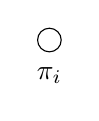
\begin{tikzpicture}
\draw[fill=white] (0,0) circle[radius=0.15];
\draw (0,-0.45) node {$\pi_i$};
\end{tikzpicture}
\end{center}
\item Draw $n_{ij}$ lines between the circles representing the roots $\pi_i$ and $\pi_j$;
\begin{center}
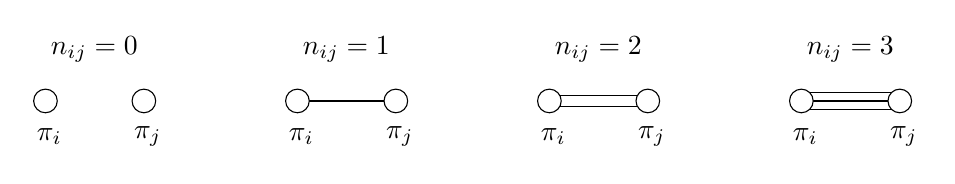
\begin{tikzpicture}
\draw (3.2,0) -- (3.2+1.25,0);
\draw (2*3.2,0.07) -- (2*3.2+1.25,0.07);
\draw (2*3.2,-0.07) -- (2*3.2+1.25,-0.07); 
\draw (3*3.2,0.11) -- (3*3.2+1.25,0.11); 
\draw (3*3.2,0) -- (3*3.2+1.25,0); 
\draw (3*3.2,-0.11) -- (3*3.2+1.25,-0.11); 
\foreach \x in {0,1,2,3} {
\draw (3.2*\x+0.62,0.65) node {$n_{ij}=\x$};
\draw (3.2*\x+0.05,-0.45) node {$\pi_i$};
\draw (3.2*\x+1.3,-0.45) node {$\pi_j$};
\draw[fill=white] (3.2*\x,0) circle[radius=0.15];
\draw[fill=white] (3.2*\x+1.25,0) circle[radius=0.15];
}
\end{tikzpicture}
\end{center}
\item If $n_{ij}=2$ or $3$, draw an arrow on the lines from the longer root to the shorter root.
\begin{center}
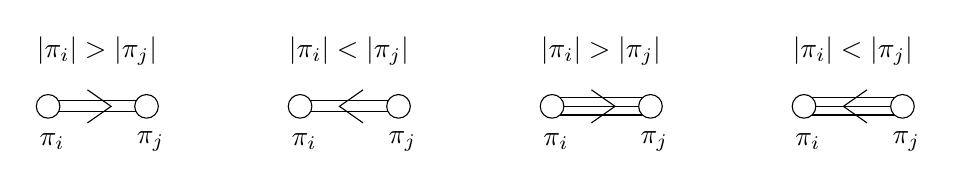
\begin{tikzpicture}
\foreach \x in {0,1} {
\draw (2*3.2*\x+0.62,0.7) node {$|\pi_i|>|\pi_j|$};
\draw (2*3.2*\x+0.65-0.15,0.21) -- (2*3.2*\x+0.65+0.15,0) -- (2*3.2*\x+0.65-0.15,-0.21);
\draw (2*3.2*\x+3.2+0.62,0.7) node {$|\pi_i|<|\pi_j|$};
\draw (2*3.2*\x+3.2+0.65+0.15,0.21) -- (2*3.2*\x+3.2+0.65-0.15,0) -- (2*3.2*\x+3.2+0.65+0.15,-0.21);
\draw (\x*3.2,0.07) -- (\x*3.2+1.25,0.07);
\draw (\x*3.2,-0.07) -- (\x*3.2+1.25,-0.07); 
}
\foreach \x in {2,3} {
\draw (\x*3.2,0.11) -- (\x*3.2+1.25,0.11); 
\draw (\x*3.2,0) -- (\x*3.2+1.25,0); 
\draw (\x*3.2,-0.11) -- (\x*3.2+1.25,-0.11); 
}
\foreach \x in {0,1,2,3} {
\draw (3.2*\x+0.05,-0.45) node {$\pi_i$};
\draw (3.2*\x+1.3,-0.45) node {$\pi_j$};
\draw[fill=white] (3.2*\x,0) circle[radius=0.15];
\draw[fill=white] (3.2*\x+1.25,0) circle[radius=0.15];
}
\end{tikzpicture}
\end{center}
\een
\ed
Dynkin diagrams completely characterise any set of fundamental roots, from which we can reconstruct the entire root set by using the Weyl transformations. The root set can then be used to produce a Cartan-Weyl basis.

We are now finally ready to state the much awaited classification theorem.
\begin{theorem}[Killing, Cartan]\index{Cartan classification}
Any simple finite-dimensional complex Lie algebra can be reconstructed from its set of fundamental roots $\Pi$, which only come in the following forms. 
\ben[label=\roman*)]
\item There are $4$ infinite families
\begin{center}
\def\arraystretch{2.5}
\setlength\tabcolsep{15pt}
\begin{tabular}{ccc}
$A_n$ & $n \geq 1$ & 
\begin{tikzpicture}[baseline={($ (current bounding box.center) - (0,3pt) $)}]
\draw (0,0) edge (2*1.25,0);
\draw (2*1.25,0) edge[dashed] (3*1.25,0);
\draw (3*1.25,0) edge (4*1.25,0);
\foreach \x in {0,1,2,3,4} {
\draw[fill=white] (1.25*\x,0) circle[radius=0.15];
}
\end{tikzpicture}\\
$B_n$ & $n \geq 2$ & 
\begin{tikzpicture}[baseline={($ (current bounding box.center) - (0,3pt) $)}]
\draw (0,0) edge (2*1.25,0);
\draw (2*1.25,0) edge[dashed] (3*1.25,0);
\draw (3*1.25+0.65-0.15,0.21) -- (3*1.25+0.65+0.15,0) -- (3*1.25+0.65-0.15,-0.21);
\draw (3*1.25,0.07) -- (4*1.25,0.07);
\draw (3*1.25,-0.07) -- (4*1.25,-0.07); 
\foreach \x in {0,1,2,3,4} {
\draw[fill=white] (1.25*\x,0) circle[radius=0.15];
}
\end{tikzpicture}\\
$C_n$ & $n \geq 3$ & 
\begin{tikzpicture}[baseline={($ (current bounding box.center) - (0,4pt) $)}]
\draw (0,0) edge (2*1.25,0);
\draw (2*1.25,0) edge[dashed] (3*1.25,0);
\draw (3*1.25+0.65+0.15,0.21) -- (3*1.25+0.65-0.15,0) -- (3*1.25+0.65+0.15,-0.21);
\draw (3*1.25,0.07) -- (4*1.25,0.07);
\draw (3*1.25,-0.07) -- (4*1.25,-0.07); 
\foreach \x in {0,1,2,3,4} {
\draw[fill=white] (1.25*\x,0) circle[radius=0.15];
}
\end{tikzpicture}\\[10pt]
$D_n$ & $n \geq 4$ & 
\begin{tikzpicture}[baseline={($ (current bounding box.center) - (0,3pt) $)}]
\draw (0,0) edge (2*1.25,0);
\draw (2*1.25,0) edge[dashed] (3*1.25,0);
\draw (3*1.25,0) -- (4*1.25,0.7);
\draw (3*1.25,0) -- (4*1.25,-0.7); 
\foreach \x in {0,1,2,3} {
\draw[fill=white] (1.25*\x,0) circle[radius=0.15];
}
\draw[fill=white] (1.25*4,0.7) circle[radius=0.15];
\draw[fill=white] (1.25*4,-0.7) circle[radius=0.15];
\end{tikzpicture}
\end{tabular}
\end{center}
where the restrictions on $n$ ensure that we don't get repeated diagrams (the diagram $D_2$ is excluded since it is disconnected and does not correspond to a simple Lie algebra)

\item five exceptional cases

\begin{center}
\def\arraystretch{2.5}
\setlength\tabcolsep{15pt}
\begin{tabular}{cl}
$E_6$  & 
\begin{tikzpicture}[baseline={($ (current bounding box.south) + (0,1pt) $)}]
\draw (0,0) edge (4*1.25,0);
\draw (2*1.25,0) edge (2*1.25,1.25);
\foreach \x in {0,1,2,3,4} {
\draw[fill=white] (1.25*\x,0) circle[radius=0.15];
}
\draw[fill=white] (2*1.25,1.25) circle[radius=0.15];
\end{tikzpicture}\\[5pt]
$E_7$ & 
\begin{tikzpicture}[baseline={($ (current bounding box.south) + (0,1pt) $)}]
\draw (0,0) edge (5*1.25,0);
\draw (2*1.25,0) edge (2*1.25,1.25);
\foreach \x in {0,1,2,3,4,5} {
\draw[fill=white] (1.25*\x,0) circle[radius=0.15];
}
\draw[fill=white] (2*1.25,1.25) circle[radius=0.15];
\end{tikzpicture}\\[5pt]
$E_8$ &  
\begin{tikzpicture}[baseline={($ (current bounding box.south) + (0,1pt) $)}]
\draw (0,0) edge (6*1.25,0);
\draw (2*1.25,0) edge (2*1.25,1.25);
\foreach \x in {0,1,2,3,4,5,6} {
\draw[fill=white] (1.25*\x,0) circle[radius=0.15];
}
\draw[fill=white] (2*1.25,1.25) circle[radius=0.15];
\end{tikzpicture}\\
$F_4$ & 
\begin{tikzpicture}[baseline={($ (current bounding box.center) - (0,3pt) $)}]
\draw (0,0) edge (1.25,0);
\draw (2*1.25,0) edge (3*1.25,0);
\draw (1*1.25+0.65-0.15,0.21) -- (1*1.25+0.65+0.15,0) -- (1*1.25+0.65-0.15,-0.21);
\draw (1*1.25,0.07) -- (2*1.25,0.07);
\draw (1*1.25,-0.07) -- (2*1.25,-0.07); 
\foreach \x in {0,1,2,3} {
\draw[fill=white] (1.25*\x,0) circle[radius=0.15];
}
\end{tikzpicture}\\
$G_2$ & 
\begin{tikzpicture}[baseline={($ (current bounding box.center) - (0,3pt) $)}]
\draw (0,0) edge (1.25,0);
\draw (0.65-0.15,0.21) -- (0.65+0.15,0) -- (0.65-0.15,-0.21);
\draw (0,0.11) -- (1.25,0.11);
\draw (0,-0.11) -- (1.25,-0.11); 
\foreach \x in {0,1} {
\draw[fill=white] (1.25*\x,0) circle[radius=0.15];
}
\end{tikzpicture}
\end{tabular}
\end{center}
\een
and no other. These are all the possible (connected) Dynkin diagrams.
\end{theorem}

At last, we have achieved a classification of all simple finite-dimensional complex Lie algebras. The finite-dimensional semi-simple complex Lie algebras are direct sums of simple Lie algebras, and correspond to disconnected Dynkin diagrams whose connected components are the ones listed above.


